\chapter{Results and Analysis}
\label{ch:resultsAndAnalysis}


% \engExpl{Sometimes this is split into two chapters.\\Keep in mind: How you are going to evaluate what you have done? What are your metrics?\\Analysis of your data and proposed solution\\Does this meet the goals which you had when you started?}


This chapter will present and analyse the results of the research conducted in this thesis.


% \sweExpl{I detta kapitel presenterar vi resultaten och diskutera dem.\\Ibland delas detta upp i två kapitel.\\Hur du ska utvärdera vad du har gjort? Vad är din statistik?\\Analys av data och föreslagen lösning\\Innebär detta att uppfyllelse av de mål som du hade när du började?}


% \sweExpl{Huvudsakliga resultat}


\section{Feasibility of building an AI assistant on open source technologies}


One of the goals of the research in this thesis was, as outlined in section~\ref{sec:goals}, to assess the feasibility of building an AI-assistant on open-source technologies and deploying the agent in an academic setting. This section will outline the results and showcase the impact open source tooling had on the implementation of the AI assistant.


\subsection{How popular was the system}


The system was developed during the spring of 2024 and gradually deployed to seven real courses at KTH starting on the 18th of April 2024. The students in the courses that participated in the study held a total of 656 chats. As can be seen in figure~\ref{fig:usage_01_cumulative_number_of_chats} these steadily increased through over the course of the study as students initiated new chats with the assistant.


\begin{figure}[H]
    \centering
    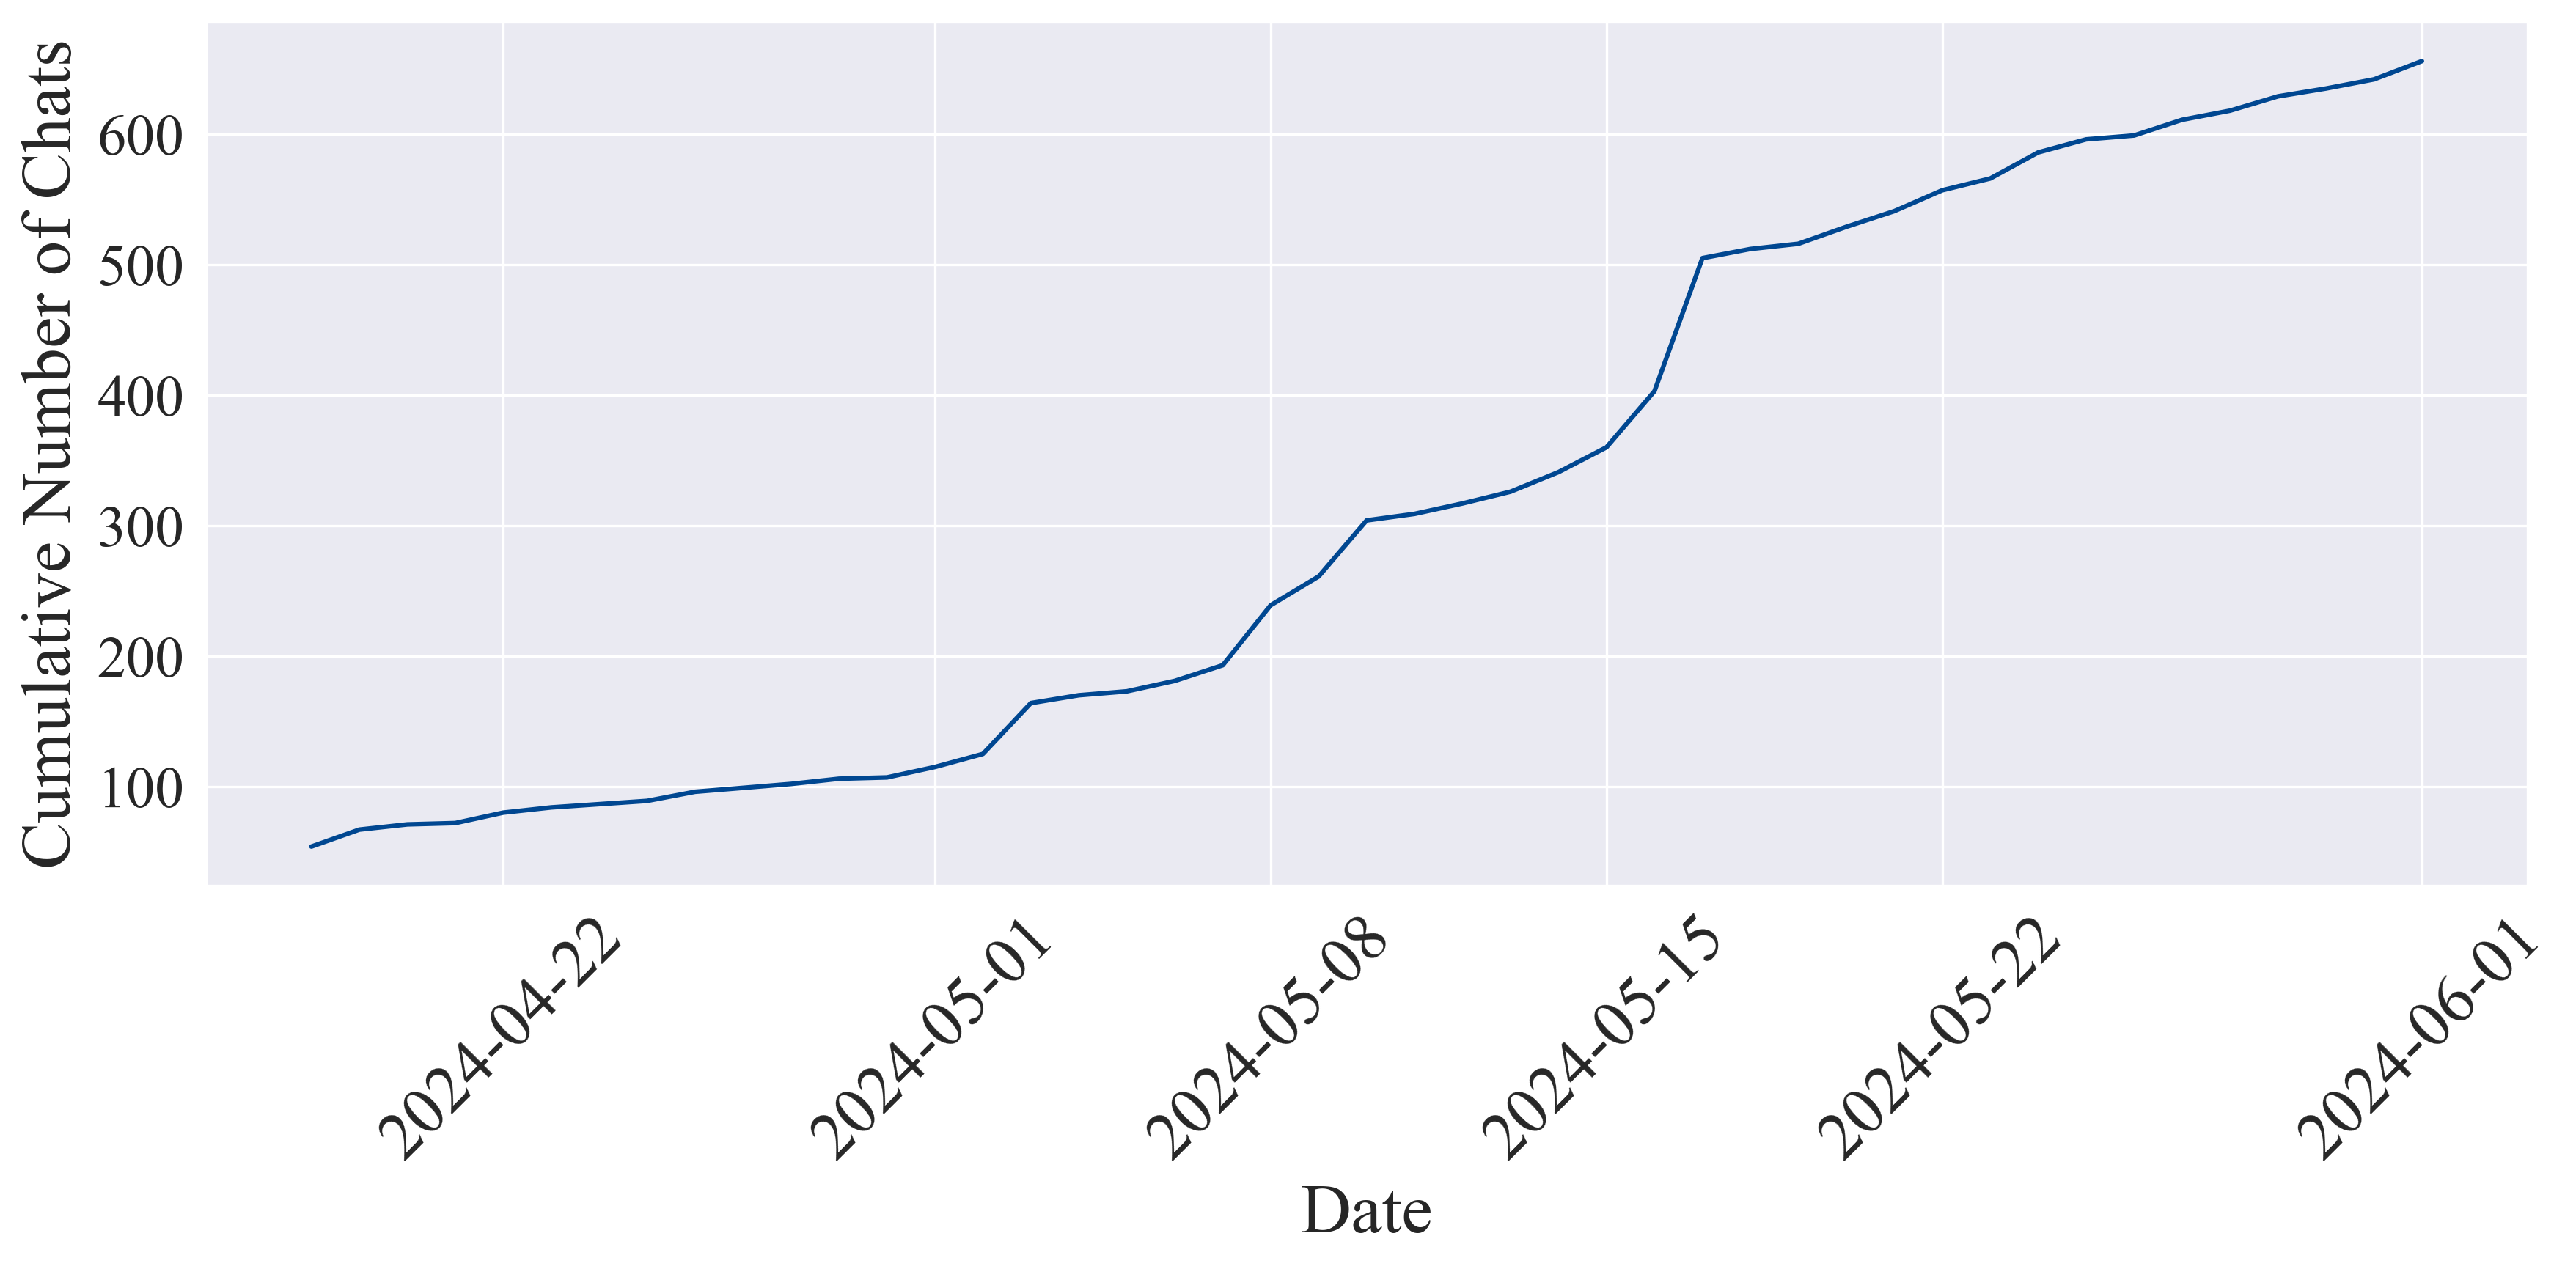
\includegraphics[width=1\textwidth]{results/plots/assets/usage-01-cumulative-number-of-chats.png}
    \caption{Cumulative number of chats started by users participating in the study}
    \label{fig:usage_01_cumulative_number_of_chats}
\end{figure}


Separating the chats initiated in the separate course rooms we observe that some courses followed a fairly linear increase in the number of chats. One example of this is the course \textit{MG2040 Assembly Technology 6.0 credits}, which can be seen in figure~\ref{fig:usage_02_cumulative_number_of_chats_per_course}.


\begin{figure}[H]
    \centering
    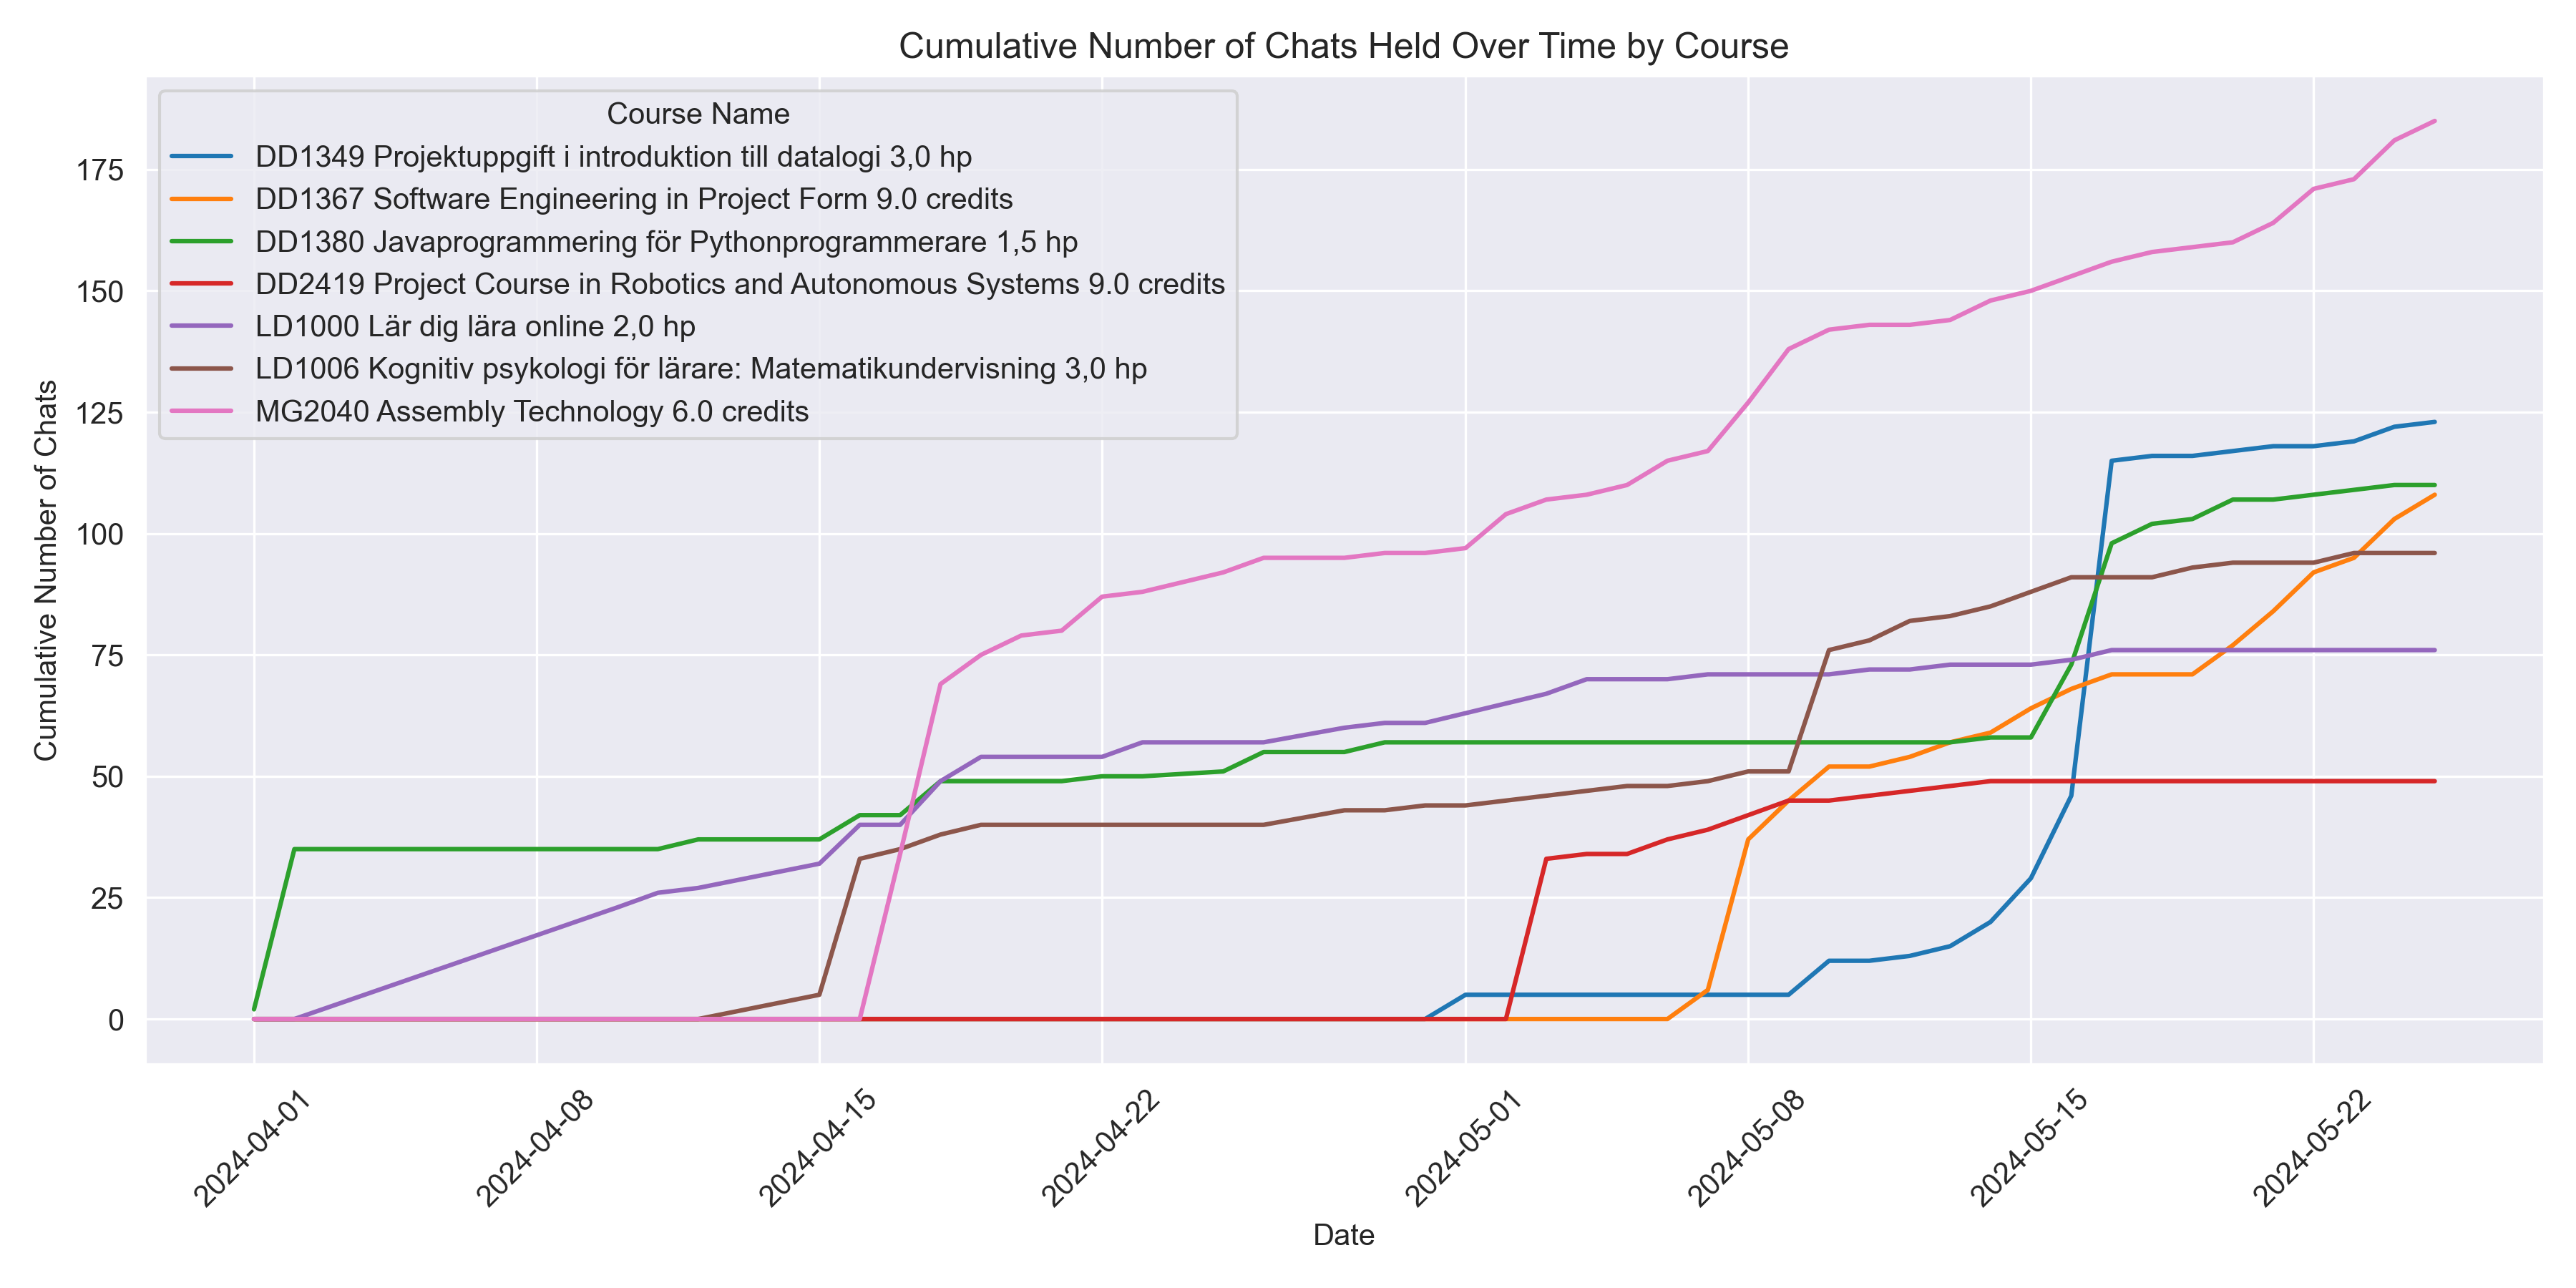
\includegraphics[width=\textwidth]{results/plots/assets/usage-02-cumulative-number-of-chats-per-course.png}
    \caption{Cumulative number of chats started by users participating in the study in each course}
    \label{fig:usage_02_cumulative_number_of_chats_per_course}
\end{figure}


Looking at other courses in figure~\ref{fig:usage_02_cumulative_number_of_chats_per_course} we can see that not all courses follow the same pattern as \textit{MG2040}. Some courses initially have very few chats. This is because the chatbot wasn’t deployed to all courses at the same time.


\subsection{Open source v. Proprietary LLMs}


\subsection{Open source v. Proprietary Embedding functions}


\section{The impact of different LLM models on the speed, accuracy and reliability of responses}


This section will present and analyse the gathered data on user preference and technological efficacy of different tools and technologies such as different \gls{RAG} toolchains and \gls{LLM}, as outlined in section~\ref{sec:goals}.


\section{Qualitative analysis of user responses}


This section will present an analysis of the free text answers users have provided in the forms that have been presented in the participating courses.




% \sweExpl{Lite statistik av fördröjningsmätningarna visas i Tabell~\ref{tab:delayMeasurements}. Förseningen har beräknats från den tidpunkt då begäran GET tas emot fram till svaret skickas.}


\section{Reliability Analysis}


% \sweExpl{Analys av tillförlitlighet\\
% Tillförlitlighet i metod och data}


\section{Validity Analysis}


% \sweExpl{Analys av validitet\\
% Validitet i metod och data}


\cleardoublepage